\chapter{EPOS}
\label{ch:epos}

%falar talvez do estilo do código (_asdf é private, etc).
%epos mote
%cite some works that used EPOS (specially giovani's).


%source: http://epos.lisha.ufsc.br/EPOS+User+Guide
EPOS (Embedded Parallel Operating System) é um sistema operacional orientado a aplicação, cujo design chama-se ADESD (\emph{Application-Driven Embedded System Design Method}), proposto por Fröhlich \cite{guto_thesis}. A ideia central do EPOS é prover um sistema operacional mínimo, de modo a minimizar o \emph{overhead} da existência de um sistema operacional, deixando o processador livre para executar a aplicação do desenvolvedor \cite{epos_user_guide}.

Como o objetivo é criar um ambiente em que o desenvolvedor possa rapidamente produzir suas aplicações, EPOS provê vários utilitários comumente usados em aplicações, como filas, listas, tabelas de hashs, vetores, semáforos, OStream (para imprimir na tela), números aleatórios, cálculo de CRC e etc. Além destes utilitários, EPOS também provê uma série de componentes como threads, alarmes, cronometros, \emph{heaps} e meios para acessar a rede (internet).

\section{Arquitetura do EPOS}


\textbf{Linguagem e paradigma:} O EPOS é escrito em C++, e não em C, como é tradicionalmente feito. Como paradigma, é usado orientação à objetos, então cada componente do EPOS está encapsulado por uma classe (como a heap, timer, thread, etc). No EPOS também é muito usado conceitos como herança e metaprogramação estática (que será abordado mais a frente).

\textbf{Mediadores de Hardware:} Dentro da arquitetura do EPOS há o conceito de mediadores de hardware, que são os componentes (ou classes) dependentes de plataforma. Idealmente, as únicas classes que precisam ser modificadas e/ou reimplementadas são os mediadores. Há mediadores específicos da placa, como para a Pandaboard, a Zedboard e etc; abstraídos sob o nome de \emph{machine} e mediadores específicos de um processador, abstraídos sob o nome de \emph{architecture}. No código do EPOS, estes mediadores encontram-se nas pastas \emph{mach} e \emph{arch}.
% Fonte: Hardware Mediators: A Portability Artifact for Component-based Systems
% HAL vs Virtualização vs Mediadores

Mediadores de hardware são uma alternativa ao tradicional uso de VMs\footnote{Virtual Machines.} e de HAL\footnote{Hardware Abstraction Layer}, proposta por Fröhlich em seu trabalho \emph{Application-Oriented System Design} \cite{guto_thesis}. O problema do uso de VMs é o seu \emph{overhead} causado devido à tradução das operações da VM em código nativo. Já o uso de um HAL incorre no problema da manutenibilidade e dificuldade de adapção à novas arquiteturas muito distintas entre si \cite{hw_mediators}. O HAL não conseguiu passar pela ``prova do tempo'', e já está sendo considerado obsoleto por distribuições GNU/Linux populares, como o 
Ubuntu \cite{linux_magazine}, sendo chamado de ``uma grande não-manutenível bagunça monolítica'' \cite{halsectomy}.

%\textbf{Interface Infladas: } Um conceito importante da arquitetura do EPOS é a Interface Inflada. %http://www.inf.ufsc.br/~guto/publications/aoos.pdf
%Em sistemas orientados a aplicação, famílias de abstrações são frequentemente tratadas como entidades únicas, algo que pode ser vantajoso para o programador da aplicação, já que este não precisaria se preocupar com qual membro em específico desta família ele precisaria usar \cite{guto_thesis}.

%Interface inflada basicamente é uma interface que declara os métodos de todas as classes que derivam dela, exportanto assim todos os métodos daquela família de abstrações, como mostra a figura \ref{fig:inflated}. Deste modo, o desenvolvedor de aplicativo poderia escrever a aplicação inteira em termos da interface inflada, relegando a tarefa de configuração do sistema a um utilitário automatizado. Tal utilitário poderia, através de uma análise sintática do código fonte, escolher quais os membros mais apropriados da família exportada serão associados no momento da compilação \cite[p.~56]{guto_thesis}.

%\begin{figure}[ht!]
%	\label{fig:inflated}
%    \centering
%    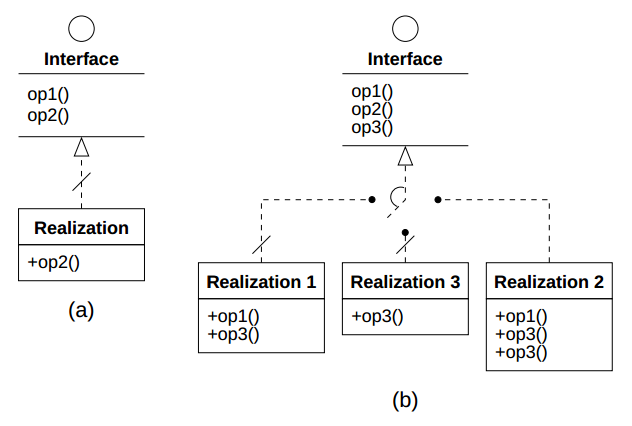
\includegraphics[width=7.5cm]{figuras/inflated_interface}
%    \caption{Exemplos de uso de interfaces infladas \cite{guto_thesis}.}
%\end{figure}


%%%%%


\section{Modos de Compilação}

Para compilar o EPOS, usa-se a ferramenta \verb+make+, através de um conjunto de \verb+makefiles+. As configurações referentes à compilação podem ser encontradas no arquivo \verb+makedefs+, onde pode-se mudar o \emph{cross compiler} a ser usado, o modo de compilação (que será descrito a seguir), arquitetura desejada e etc.


O EPOS pode ser compilado de três formas diferentes:

\begin{description}
\item[Library] O sistema é compilado junto com a aplicação, sem distinção de espaço de endereçamento, existência de modo usuário nem chamadas de sistema.
\item[Builtin] Semelhante ao \emph{library}, com a diferença de que o SO é colocado nos endereços mais altos, e a aplicação nos endereços mais baixos (ambos ainda usam o mesmo espaço de endereçamento), em contraste ao \emph{library} que mistura os dois. O principal uso desse modo é para depuração e desenvolvimento \cite{EPOS}.
\item[Kernel] Existe dois espaços de endereçamento diferentes, com modo usuário e kernel, com uma interface de chamada de sistema entre eles. Existe o conceito de \emph{task}.

\end{description}

%tools
Durante o processo de compilação do EPOS, duas ferramentas próprias são chamadas: \verb=eposcc= e \verb=eposmkbi=. O \verb=eposcc= é um \emph{script} auxiliar do processo de compilação, é nele em que é diferenciado o modo de compilação do EPOS, e é nele que é acertada a ordem de ligação (\emph{linkage}) dos construtores globais do EPOS, algo muito importante para a inicialização do SO, como é descrito na seção \ref{sec:inicializacao}.
Já o \verb=eposmkbi= é uma ferramenta cujo objetivo é criar uma imagem ``bootável'' do SO com a aplicação. Esta imagem é uma imagem de virtualização de disco, com as metainformações necessárias já adicionadas a ela \cite{tarcisio}. Estas metainformações são adicionadas também à \verb=struct= \verb+System_info+, para que seja posteriormente usada pelo EPOS durante sua inicialização.



\section{Inicialização}
\label{sec:inicializacao}
O EPOS inicia executando um conjunto de códigos escritos em assembly, chamados de crts.
No crt, a primeira tarefa feita na inicialização do EPOS é a configuração das pilhas do sistema. Feito isto, o EPOS trata de limpar a seção .bss, para futuro reuso.
Antes de ser chamado o construtor dos demais objetos globais, a UART e Display são inicializados, assim é possível mais facilmente depurar o código dos construtores.
Então o EPOS começa a chamar o construtor global de cada componente do sistema. O crt consegue localizar onde está localizado cada construtor devido à forma como o EPOS foi compilado e ligado (\emph{linked}). A figura \ref{fig:initialization} ilustra num diagrama de sequência a ordem de construção dos objetos globais.

\fig{0.58}{initialization}{Diagrama de sequência da inicialização do EPOS}

Primeiro é construído o \verb+First_Object+, cuja principal função é apenas ser um ponto de entrada conhecido para o primeiro objeto do sistema.
Em seguida, é construído \verb+Init_System+. É neste construtor que todos os mediadores de hardware são construídos, com exceção da UART que já foi previamente construída no crt. Neste construtor, primeiramente é inicializado o \emph{timer}, MMU, e, se disponível, o TSC (\emph{Time Stamp Counter}). Em seguida o construtor aloca uma porção de memória para futuro uso da heap do sistema. Feito isto, o SCU (\emph{Snoop Control Unit}), tratador de interrupções e alarme são também construídos.

\verb+Init_Application+ é responsável por alocar a heap da aplicação, através da requisição de páginas da MMU. \verb+Init_First+ chama o inicializador das \emph{threads}, que então inicializa a \emph{thread} da aplicação e a \emph{idle thread}, que é uma \emph{thread} especial que é executada quando o escalonador não encontra outra \emph{thread} pronta para executar. Em seguida à criação destas \emph{threads}, é chamado \verb+context->load()+ da \emph{thread} da aplicação, fazendo com que o fluxo de execução seja finalmente transferido para a aplicação.

\section{Traits}
\label{sec:traits}
Existem 4 arquivos \verb=traits.h= que devem ser levados em consideração em um porte, dois deles devem ser completamente reescritos. Os arquivos \verb+./include/traits.h+ e \verb+/include/system/traits.h+ (onde `.' é a pasta raiz do código) possuem configurações gerais do EPOS, que, a princípio, devem ser independentes de arquitetura. Na prática há alguns pequenos ajustes que devem ser feitos nesses arquivos, pois é lá que se define, por exemplo, se o EPOS trabalhará em um processador \emph{multicore}, se utilizará \emph{scratchpad}, quais componentes estarão em modo de depuração e etc; entretanto isto se resume a trocar o valor de algumas variáveis de \emph{true} para \emph{false} e vice-versa.

Os outros dois arquivos são \verb+./include/mach/zynq/traits.h+ e\\ \verb+./include/arch/armv7/traits.h+. Essa divisão é necessária pois, como dito anteriormente, é possível de um mesmo processador estar em diferentes \emph{machines}, e, caso seja necessário fazer um porte para aquela plataforma, bastaria modificar os arquivos da pasta \emph{mach}, deixando os da pasta \emph{arch} praticamente intactos, o que facilita novos portes.

O arquivo \verb+./include/arch/armv7/traits.h+ trata das opções específicas do processador, portanto é lá que opções como \emph{endianess}, velocidade de \emph{clock}, número de \emph{cores}, tamanho da \emph{heap} e \emph{stacks}, bem como outras opções pertinentes ao mapeamento de memória e opções da MMU podem ser configuradas.

No arquivo de \verb=traits= da \emph{machine}, ficam as opções de configuração de componentes como a UART, controlador de interrupções, \emph{timer}, e qualquer componente de interfaceamento externo à placa (rede, por exemplo). Componentes podem ser facilmente ativados ou desativados nestas opções.

\section{Interrupções}


Como o EPOS foca no desempenho da aplicação, em seu design opta-se por utilizar a menor quantidade possível de interrupções, e evitá-las sempre que possível, isto contribui também para que o sistema seja mais previsível. Se a aplicação não precisar de componentes específicos que necessitem interrupções (como um rádio, por exemplo), a única interrupção a ser tratada será a do \emph{timer}, já que o escalonador e alarm necessitam dele.

%interrupções (indexação de um vetor de interrupções pelo seu ID)
%exception -> ic_handler -> timer_handler -> alarm handler
%                                         -> scheduelr handler

A sequência de chamadas de função, dado o recebimento de uma interrupção de \emph{timer} está ilustrada na figura \ref{fig:exception_handling}. Exception é um código em assembly cujo objetivo é salvar o contexto no recebimento da chamada, chamar o tratador de interrupções padrão, e restaurar o contexto após isto. O tratador de interrupções do \emph{interrupt controller} (IC) possui um vetor de tratadores de interrupção, onde para cada número de interrupção, há uma entrada correspondente no vetor. Este tratador então lê o registrador responsável por armazenar o número da interrupção gerada (esta parte é dependente de arquitetura, na Zedboard uma interrupção de timer tem número 29, por exemplo), indexa seu vetor e chama o tratador apropriado. Chegando no tratador do \emph{timer}, este chama os tratadores de todos os componentes que dependem de um \emph{timer}, neste caso o \verb+Alarm+ e \verb+Scheduler+.

\fig{0.17}{exception_handling}{Sequência de chamada de tratadores de interrupção. A interrupção gerada neste exemplo foi uma de \emph{timer}.}. 



\section{Gerenciamento de Memória}
\label{sec:gerenciamento}
Uma das principais funções de um sistema operacional é o gerenciamento de memória. Isto inclui organizar a memória (mapeamento de memória, definição do que cada região da memória guarda, etc) e gerenciamento (manter registro de páginas livres, definir permissões, etc).

% MMU::alloc
Para entendermos como isto é feito, primeiro é necessário entendermos como funciona a abstração da MMU no EPOS. Isto se dá com 4 classes principais, a \verb+ARMv7_MMU+, que possui a lista de memórias livres, a \verb+Page_Table+, que mapeia porções de até 1MB de endereço virtual para físico, \verb+Chunk+, que nada mais é que um conjunto de \verb+Page_Tables+, e, finalmente, \verb+Directory+, que é um conjunto de \verb+Chunks+ (ou \verb+Page_Tables+).

A classe \verb+ARMv7_MMU+ possui uma uma lista de porções de memórias livres, gerenciadas pelas funções \verb+alloc+ e \verb+free+. A granularidade destas porções de memória é a de \emph{frames}
\footnote{Frame é uma porção de tamanho fixo de memória física (normalmente 4KB). A diferença entre uma página e um frame é que um frame refere-se à uma porção da memória física, enquanto uma página refere-se à uma porção de memória virtual.}.
Note que esta lista utiliza os endereços \textbf{físicos} destas porções de memória.

A tabela de páginas da MMU do ARMv7, assim como a do IA32, possui dois níveis. Na nomenclatura da ARM, a tabela de nível mais alto é a tabela L1 (de \emph{level}), onde cada entrada desta tabela aponta para outra tabela (uma tabela L2).
Cada entrada da tabela L2 possui o endereço físico correspondente ao endereço virtual requisistado. A maneira como esta tabela é usada para traduzir um endereço virtual para um físico varia de arquitetura para arquitetura, sendo esta parte explicada detalhadamente na seção \ref{sec:mmu}.

Nas abstrações do EPOS, a classe que gerencia a tabela L2 é a \verb+Page_Table+, e a classe que gerencia a tabela L1 é a \verb+Directory+. Portanto uma \verb+Page_Table+ é apenas um vetor, onde em cada posição está escrita uma posição de memória física, junto de algumas \emph{flags} (que definem permissões, ``cacheabilidade'' e etc). O número máximo de entradas numa \verb+Page_Table+ é dependente de arquitetura. No ARMv7 são 256 entradas de 4 bytes (mapeando até 1MB de memória portanto), e no IA32 são 1024 entradas (que mapeiam até 4MB), cada página (\emph{frame}) possuindo 4 KB.

\verb+Chunk+ é uma classe bastante importante, e, apesar de simples, é importante que se tenha um bom entendimento sobre como ela funciona.
Cria-se um \verb+chunk+ para alocar uma certa porção de memória, em um espaço de endereçamento próprio. 

Esta classe recebe dois parâmetros: A quantidade de bytes a serem alocados, e as \emph{flags} a serem usadas. \verb+Chunk+ então calcula quantas tabelas de páginas serão necessárias para mapear a quantidade de bytes requisitada, e então cria estas páginas contiguamente no espaço de endereçamento virtual (em qualquer lugar da memória, a ser decidido pela função \verb+alloc+).

\verb+Chunk+ então chama a função \verb+map+ de \verb+Page_Table+ para mapear aquela porção da memória. Cada \emph{frame} é requisitado pela função \verb+alloc+, o que significa que cada \verb+Page_Table+ pode estar apontando para qualquer posição da memória, não estando os \emph{frames} necessariamente contiguos na memória física, apesar que eles serão \textbf{contíguos} no espaço de memória virtual mapeada num mesmo \verb+Chunk+.

Portanto esta classe efetivamente aloca uma porção de memória em um espaço de endereçamento próprio, este fato será bastante importante quando discutirmos a criação das \emph{heaps} de usuário e do sistema.

%Directory
Já a classe directory é responsável por gerenciar e unificar todas estas porções de memória. Sua principal função é a \verb+attach+, que tomando como parâmetro um \verb+Chunk+, mapeia cada uma de suas páginas contiguamente (isto é, cria uma entrada em \verb=directory= que aponta para uma página criada em \verb+Chunk+, para cada página dele).

A figura \ref{fig:mmu_translation} ilustra a interação entre os conteúdos das entradas de \verb+Directory+ e \verb+Page_Table+ com a memória física. A quantidade de bits usada para indexar as tabelas é dependente de arquitetura. Aqui, os primeiros 12 bits indexam a tabela de \verb+Directory+, os 8 bits seguintes indexam a tabela de \verb+Page_Table+, e os últimos 12 bits são simplesmente copiados do endereço virtual para o físico.
Portanto, no exemplo, do endereço 0xAB2FF123, o número 0xAB2 será usado para indexar a tabela de nível 1 (\verb=Directory=), o número 0xFF indexará a tabela de segundo nível (\verb+Page_Table+), onde estará escrito o endereço físico correspondente àquele endereço virtual.
Mais detalhes sobre este processo na seção \ref{sec:mmu}, em particular na imagem \ref{fig:translation}.


\fig{0.45}{mmu_translation}{Interação entre Directory e Page\_Table com a memória física. Neste exemplo, o endereço virtual 0xAB2FF123 seria traduzido para o endereço físico 0xDEAD1123. A última posição de memória física indexável neste exemplo é 0x1FFFF\_\_\_ pois a Zedboard dispõe de 512MB.}


\verb+Directory+ não sabe a qual \verb+Chunk+ uma determinada \verb+Page_Table+ pertence, e a tradução de endereços pode ocorrer independente desta informação. Na figura \ref{fig:mmu} é ilustrada a interação entre as classes discutidas.

\fig{0.20}{mmu}{Diagrama de classes da MMU.}


%make a diagram showing how MMU alloc a physical page, and how the heap lends pages that were already allocated in the MMU's point of view.

\subsection{Heaps}

A \emph{heap} é responsável por armazenar e gerenciar os dados dinâmicos criados durante a execução da aplicação e do SO (a cada \verb+malloc/new+ executado, por exemplo). Existem duas heaps: A do sistema, e a do usuário. É possível compilar o EPOS com apenas a \emph{heap} do sistema, quando o desenvolvedor decide que a aplicação deverá rodar em modo privilegiado, não sendo usado portanto o modo usuário (isto é configurável nos \verb+traits+).

A memória da \emph{heap} é alocada através de um \verb+Chunk+. É neste ponto que pode-se atribuir \emph{flags} que limitam as permições de acesso (a \emph{heap} de usuário é alocada sem restrições de acesso, já a do sistema aloca uma porção de memória que só pode ser acessada em modo privilegiado). É por usar um \verb+Chunk+ também que do ponto de vista da aplicação, é como se ela tivesse acesso à todo o espaço de memória. Note que do ponto de vista da MMU (e sua lista de memórias livres), é como se a porção de memória da heap estivesse em uso, já a heap vê sua porção de memória como livre.

A heap trabalha com uma lista de memórias livres (igual à da MMU), só que ao contrário da MMU, que aloca somente páginas (frames) inteiros de memória, a heap aloca quantidades de memória com a granularidade de bytes.

Para que a \emph{heap} do sistema e a \emph{heap} do usuário seja corretamente usada, faz-se no EPOS \emph{overload} do operador \verb+new+ e \verb+delete+, e \emph{placement new}. Por exemplo, um \verb+new A()+ chamaria as seguintes funções:

\begin{lstlisting}
inline void * operator new(size_t bytes) {
    return malloc(bytes);
}
inline void * malloc(size_t bytes) {
    if(Traits<System>::multiheap)
        return Application::_heap->alloc(bytes);
    else
        return System::_heap->alloc(bytes);
}
\end{lstlisting}

O compilador se encarrega de avaliar o \verb+sizeof+ de \verb+A+, e envia como parâmetro para o operador \verb+new+. \verb+multiheap+ é um atributo dos \verb+traits+ que define se o sistema possui uma \emph{heap} de usuário separada da \emph{heap} do sistema ou se é usada somente uma única \emph{heap}.

Para o sistema alocar memória usando sua própria \emph{heap} com o operador \verb+new+, faz-se um \emph{overload} do \emph{placement new}, como segue:

\begin{lstlisting}
enum System_Allocator {SYSTEM};

inline void * operator new(size_t bytes, const EPOS::System_Allocator & allocator) {
    return EPOS::System::_heap->alloc(bytes);
}
\end{lstlisting}

Feito isto, para alocar, dentro do EPOS, alguma porção de memória utilizando o operador \verb+new+ com a \emph{heap} do sistema, basta escrever \verb+(SYSTEM)+ logo após o \verb+new+, por exemplo:

\begin{lstlisting}
_timer = new (SYSTEM) Alarm_Timer(handler);
\end{lstlisting}


\section{Escalonadores}

O EPOS suporta diversos escalonadores, desde os de propósito geral até escalonadores de tempo real \emph{multicore}.
Do primeiro tipo, temos o \emph{Round Robin} e \emph{First-Come, First-Served}, do segundo, \emph{Rate Monotonic}, \emph{Deadline Monotonic} e \emph{Earliest Deadline First} (global, particionado e agrupado), e também o escalonador descrito em \cite{gio}.

\fig{0.30}{edf_uml}{Diagrama de classes para os escalonadores que usam a política \emph{Earliest Dealine First} \cite[p.~184]{gio}.}

O EPOS é projetado de modo a permitir grande reuso ao se escrever um escalonador. Por exemplo, há três escalonadores que utilizam a política EDF (\emph{Earliest Deadline First}), que nada mais é que um critério de escolha de \emph{thread}, onde neste caso procura-se escolher aquela cujo \emph{dealine} está mais próximo, por isto separou-se esta parte das especificidades que existem entre os escalonadores. 

A figura \ref{fig:edf_uml} ilustra a relação entre as classes dos escalonadores que herdam de EDF.  Não é o objetivo deste trabalho entrar em detalhe nas especificidades dos diferentes escalonadores do EPOS, entretanto será colocada uma breve descrição destes três escalonadores EDF para que a figura fique clara.

\begin{description}

\item[PEDF:] O \emph{partitioned} EDF (particionado) possui uma fila de tarefas a serem escalonadas para cada processador. A escolha de que fila cada tarefa é atribuida é feita de forma estática. Cada tarefa executa sempre no mesmo processador, não havendo migração destas. 

\item[GEDF:] O EDF global utiliza uma única fila de tarefas, e atribui uma tarefa toda vez que um processador fica livre. A vantagem deste escalonador sobre o PEDF é que ele consegue escalonar conjuntos de tarefas que o PEDF não conseguiria, entretanto seu desempenho costuma ser menor e menos previsível, pois migrar uma tarefa de um processador para o outro é custoso, e gera um mal aproveitamento das memórias \emph{cache}.

\item[CEDF:] Este é o caso geral do PEDF e GEDF. Neste escalonador há uma fila para cada grupo de processadores (\emph{cluster}). Por exemplo, numa arquitetura que usa 8 processadores, poder-se-ia fazer 4 grupos de 2 processadores cada, totalizando 4 filas. Somente há migração de tarefas entre processadores de um mesmo grupo. Caso o grupo seja do tamanho do número de cores, tem-se o GEDF, e se cada grupo tiver apenas um processador, obtem-se o PEDF.

\end{description}

\section{Relação Mediadores-Abstrações}

Esta seção discute a relação entre os mediadores de hardware do EPOS (dependentes de arquitetura) com as abstrações do EPOS que usam estes mediadores (independente de arquitetura). O objetivo aqui é mostrar que estas abstrações não precisam ser alteradas entre as diferentes arquiteturas que o EPOS suporta, estando todas as diferenças arquiteturais isoladas em seus mediadores.

%Relação abstrações do epos e mediadores:
%-> Relação das abstrações do EPOS com os mediadores feitos.
%-> Imagem que víncula mediadores com a sua interface genérica
%-> Apontar que estas interfaces não precisam ser alteradas

Cada mediador de hardware (que chamaremos apenas de ``mediador'' deste ponto em diante) possui uma classe genérica que o representa. Esta classe é a mesma para todas as arquiteturas, e cada novo mediador implementado deve estender esta classe, deste modo pode-se manter a uniformidade das interfaces de cada novo mediador. Por exemplo, no caso da UART, cada novo mediador da UART precisa estender a classe \verb+UART_Common+, como ilustra a figura \ref{fig:uart_diagram}. Note que o EPOS possui suporte para diversas arquiteturas, no diagrama são colocadas apenas duas por simplicidade. A figura \ref{fig:mmu} da seção \ref{sec:gerenciamento} também ilustra isto.

\fig{0.30}{uart_diagram}{Diagrama de classes da UART.}

A resolução do mediador da-se em tempo de compilação, através de metaprogramação estática e do uso de scripts automatizados. Para escolher a arquitetura alvo para compilar o EPOS, basta alterar o arquivo de traits \verb+./include/system/traits.h+, trocando os valores das variáveis \verb+ARCH+ e \verb=MACH=. Durante o processo de compilação, usando a ferramenta \verb=sed=, o arquivo \verb=./include/system/config.h= é alterado para alterar as variáveis \verb+ARCH+ e \verb=MACH= para as escolhidas pelo usuário. Feito isto, macros são usadas para a resolução da inclusão dos \emph{headers} corretos para a arquitetura escolhida. Segue abaixo algumas destas macros:

\begin{verbatim}
#define __HEADER_ARCH(X)         <arch/ARCH/X.h>
#define __HEADER_MACH(X)         <mach/MACH/X.h>
\end{verbatim}

Para que o código independente de arquitetura do EPOS possa se referenciar às classes dos mediadores através de um nome genérico, para cada porte é feito um arquivo \verb=config.h= onde são definidos tipos com nome padronizado que se referem aos mediadores daquela arquitetura. Por exemplo, um trecho do \verb=config.h= do Zynq segue abaixo:

\begin{verbatim}
typedef ARMV7      CPU;
typedef ARMV7_MMU  MMU;
typedef Zynq       Machine;
typedef Zynq_IC    IC;
typedef Zynq_UART  UART;
typedef Zynq_Timer Timer;
\end{verbatim}

Com isto, todos os mediadores ficam abstraídos do ponto de vista do restante do sistema operacional, e podem ser trocados através da simples alteração de duas variáveis no arquivo de \verb=traits=, seguida de nova compilação.
